% Rotate a path around a point: Double Pendulum Case
% https://latexdraw.com
% 21/02/2020, 23:55

\documentclass[border=0.1cm]{standalone}
\usepackage{tikz}


\begin{document}

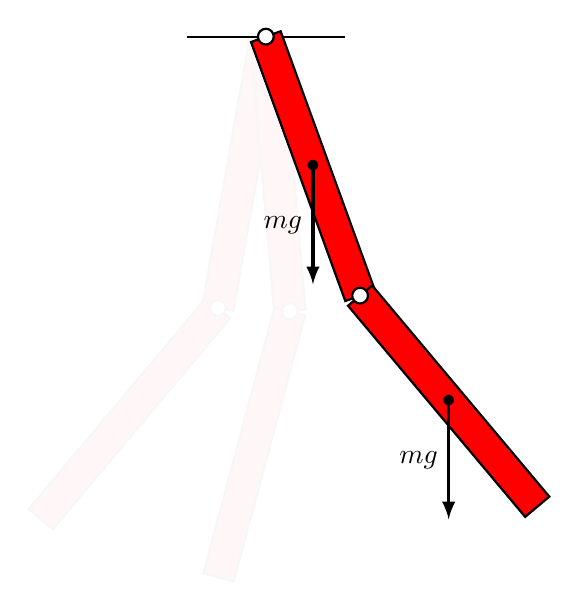
\begin{tikzpicture}[thick]

\begin{scope}[rotate=-10,black!3]
\draw[fill=red!3] (-0.2,0) rectangle (0.2,-3.5);
\draw[fill=red!3,rotate around={-30:(0,-3.5)}] (-0.2,-3.5) rectangle (0.2,-7);
\draw[fill=white] (0,-3.5) circle(0.1);
\end{scope}

\begin{scope}[rotate=5,black!3]
\draw[fill=red!3] (-0.2,0) rectangle (0.2,-3.5);
\draw[fill=red!3,rotate around={-20:(0,-3.5)}] (-0.2,-3.5) rectangle (0.2,-7);
\draw[fill=white] (0,-3.5) circle(0.1);
\end{scope}

\draw (-1,0) -- (1,0);

\begin{scope}[rotate=20]
\draw[fill=red] (-0.2,0) rectangle (0.2,-3.5) node[midway](a){$\bullet$};
\draw[fill=red,rotate around={20:(0,-3.5)}] (-0.2,-3.5) rectangle (0.2,-7)node[midway](b){$\bullet$};;
\draw[fill=white] (0,-3.5) circle(0.1);
\end{scope}

\draw[-latex,very thick] (a.center) -- ++(0,-1.5) node[midway,left]{$mg$};
\draw[-latex,very thick] (b.center) -- ++(0,-1.5) node[midway,left]{$mg$};


\draw[fill=white] (0,0) circle(0.1);

\end{tikzpicture}

\end{document}
